\subsection{Reactivity}
Asymptotic resilience governs the long-term rate of recovery. However, in the short term, perturbations can initially be amplified before eventually decaying to the stable equilibrium (Figure \ref{fig:reactivity}). Motivated by this transient behavior, an alternative measure of system response to perturbations was introduced by Neubert and Caswell in \cite{neubertAlternativesResilienceMeasuring1997a}.

\begin{figure}[ht]
	\centering
	\captionsetup{width=0.8\linewidth}
	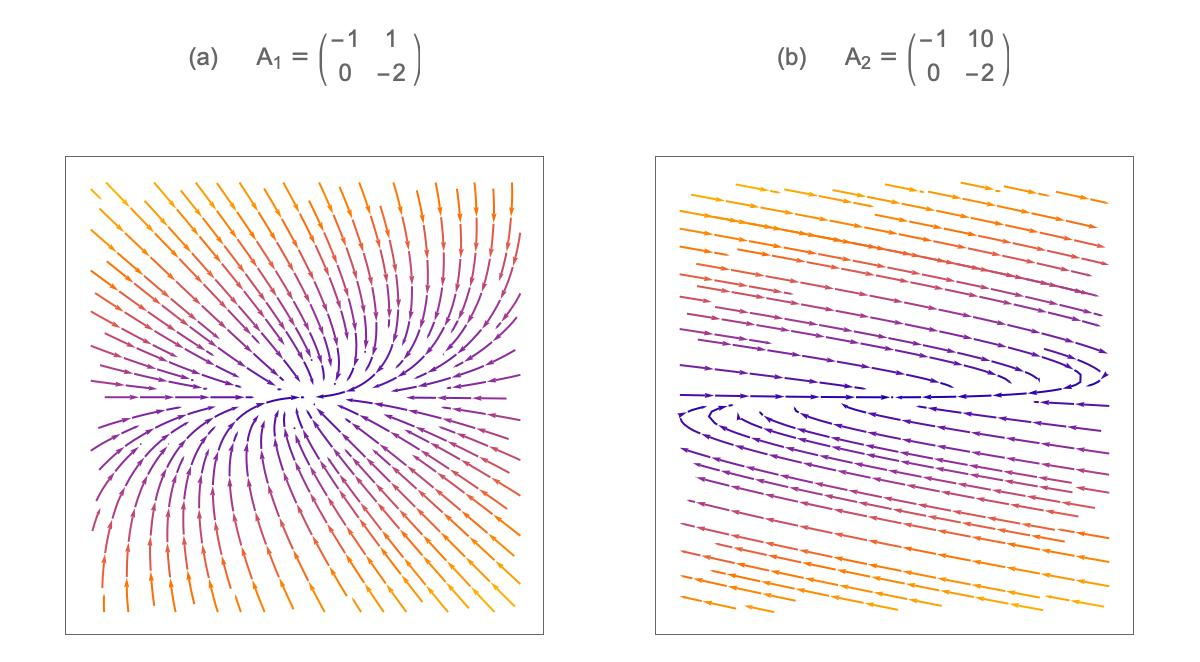
\includegraphics[width=0.8\textwidth]{figs/positive_reactivity_real_example}
	\caption{Phase portraits of two linear systems $x' = \textbf{A}x$ with the same eigenvalues  $\lambda = -1, -2$. (a) All trajectories decay monotonically in magnitude. (b) Trajectories may initially increase in magnitude. Example reproduced from \cite{neubertAlternativesResilienceMeasuring1997a}.}
	
	\label{fig:reactivity}
\end{figure} 

\begin{definition}
	Suppose that $x_\ast$ is a stable rest point of the ODE (\ref{eqn:ode}). Let $\textbf{A} = Df(x_\ast)$ be the Jacobian, and let $\textbf{H} = \frac{\textbf{A}+\textbf{A}^T}{2}$ be its symmetric part. Since $\textbf{H}$ is a real symmetric matrix, it has real eigenvalues. Let $\lambda_1(\textbf{H})$ be the maximum eigenvalue.
	
	 \begin{center}
	 	The \textbf{reactivity} of the system at the stable rest point is $\lambda_1(\mathbf{H})$.\\ If this number is positive, the system is called \textbf{reactive}.
	 \end{center}
	
	\qed
\end{definition}

Reactivity measures the maximum possible relative rate of initial amplification. The following proposition, which relies on elementary linear algebra, shows this result for linear systems. 

\begin{proposition}[Neubert and Caswell]
	For the linear system $x' = \mathbf{A}x$, $\lambda_1(\mathbf{H}) = \max\limits_{x\in \mathbb{R}^n \setminus \{0\}} \dfrac{||x||'}{||x||}$.
\end{proposition}

\begin{proof}	
	\begin{align*}
		\dfrac{||x||'}{||x||} 	&= \dfrac{1}{||x||} \dfrac{d}{dt}\big(x^Tx\big)^{1/2} \\
										&= \dfrac{1}{2||x||^2} (x^T x' + (x')^T x) \\
										&=  \dfrac{1}{2||x||^2} (x^T \mathbf{A}x + x^T\textbf{A}^Tx) \\
										&= \dfrac{ x^T\mathbf{H}x}{||x||^2}
	\end{align*}

	This expression is a scale invariant function of $x$, so to maximize it, we only need to consider unit vectors. $$\max\limits_{||x||=1} x^T \mathbf{H} x$$
	%
	
	$\mathbf{H}$ is real symmetric, hence diagonalizable with an orthogonal change of basis. Let $\{\lambda_1, \lambda_2, \ldots \lambda_n\} = spec(\mathbf{H})$, in order from largest to smallest.
	\begin{align*}
		x^T\mathbf{H}x &= x^T(\mathbf{BDB}^T)x\\
		&= (x^T\mathbf{B})\mathbf{D}(\mathbf{B}^Tx)\\
		&= y^T \mathbf{D}y, ~\text{  where } y = \mathbf{B}^Tx \text{ is also unit.}\\
		&= \lambda_1 y_1^2 + \lambda_2 y_2^2 + \ldots +\lambda_n y_n^2.
	\end{align*}
The maximum of this expression over all $||y||=1$ is clearly $\lambda_1$, when $y= (y_1, \ldots , y_n) =(1, 0, \ldots, 0)$.

	
	%Since $\mathbf{H}$ is a symmetric matrix, it defines a quadratic form $Q(x) = x^T \mathbf{H} x$. The maximum value of a quadratic form restricted to the unit sphere is the largest eigenvalue of its matrix representation. \todo{cite}
	
\end{proof}

%If a linear system has positive reactivity, then there are arbitrarily small perturbations that will initially amplify, before eventually decaying to the sink. 



to do: relation between nonlinear and linearized systems

%connection to SVD?

% connection to Turing instability?



